\documentclass[11pt]{beamer}
\usetheme{Warsaw}
\setbeamertemplate{page number in head/foot}{\insertframenumber /100}
\usepackage[T1]{fontenc}
\usepackage{polski}
\usepackage[utf8]{inputenc}
\usepackage[greek, polish]{babel}
\usepackage{array, multirow, epstopdf, geometry, wrapfig} 
\usepackage{amsmath,amssymb,lmodern,amsfonts}
\usepackage{graphicx}
\usepackage{caption}
\graphicspath{ {./img/} }
\author{dr inż. Szymon Maćkowiak}
\title{\textbf{Tytuł prezentacji}}
%\setbeamercovered{transparent} 
%\setbeamertemplate{navigation symbols}{} 
%\logo{
\includegraphics[height=1cm]{logo_CDV_full_colour_RGB_PL.png}}
\institute{Miejsce pracy} 
%\date{} 
%\subject{} 

%----------------------------------------------------------------------------
%wstawienie obrazka logo w prawy górny prostokąt
%----------------------------------------------------------------------------
\makeatletter
\setbeamertemplate{headline}
{%
  \leavevmode%
  \@tempdimb=2.4375ex%
  \ifnum\beamer@subsectionmax<\beamer@sectionmax%
    \multiply\@tempdimb by\beamer@sectionmax%
  \else%
    \multiply\@tempdimb by\beamer@subsectionmax%
  \fi%
  \ifdim\@tempdimb>0pt%
    \advance\@tempdimb by 1.825ex%
    \begin{beamercolorbox}[wd=.5\paperwidth,ht=\@tempdimb]{section in head/foot}%
      \vbox to\@tempdimb{\vfil\insertsectionnavigation{.5\paperwidth}\vfil}%
    \end{beamercolorbox}%
    \begin{beamercolorbox}[wd=.5\paperwidth,ht=\@tempdimb]{subsection in head/foot}%
      \vbox to\@tempdimb{\vfil\insertsubsectionnavigation{.3\paperwidth}\vfil}%
      \hfill
      
\includegraphics[height=\headheight]{logo_CDV_full_colour_RGB_PL_3}
    \end{beamercolorbox}%
  \fi%
}
\makeatother

%----------------------------------------------------------------------------
%modyfikacja domyślnej palety kolorów
%----------------------------------------------------------------------------
% CDV
\definecolor{colorA}{RGB}{1,182,221} %błękitny
\definecolor{colorB}{RGB}{254,204,40} %żółty
\definecolor{colorC}{RGB}{2,77,101} %granatowy

% PP
%\definecolor{colorA}{RGB}{1,182,221} %błękitny
%\definecolor{colorB}{RGB}{200,200,200} %żółty
%\definecolor{colorC}{RGB}{2,77,101} %granatowy

\setbeamercolor*{palette primary}{bg=colorA, fg = colorB}
\setbeamercolor*{palette secondary}{bg=colorB, fg = colorB}
\setbeamercolor*{palette tertiary}{bg=colorC, fg = colorB}
\setbeamercolor*{palette quaternary}{bg=colorC, fg = colorB}

%----------------------------------------------------------------------------
%dokument zaczyna się tutaj
%----------------------------------------------------------------------------
\begin{document}
%----------------------------------------------------------------------------
%strona tytułowa
%----------------------------------------------------------------------------
\begin{frame}
\titlepage
\end{frame}
%----------------------------------------------------------------------------
%spis treści
%----------------------------------------------------------------------------
\begin{frame}
\tableofcontents
\end{frame}
%----------------------------------------------------------------------------
%literatura
%----------------------------------------------------------------------------
\begin{frame}{Literatura}
\begin{itemize}
{\tiny
\item [1] Autor 1, {\it ,,Tytuł 1''}, \\Wydawnictwo, Miasto, rok
\item [2] Autor 1, {\it ,,Tytuł 2''}, \\Wydawnictwo, Miasto, rok
\item [3] Autor 1, {\it ,,Tytuł 3''}, \\Wydawnictwo, Miasto, rok



}
\end{itemize}
\end{frame}
%----------------------------------------------------------------------------
%nowa sekcja
%----------------------------------------------------------------------------
\section{Tytuł sekcji}
%----------------------------------------------------------------------------
\begin{frame}{Opis slajcu}
\begin{minipage}[0.5\textheight]{\textwidth}
\begin{columns}[T]

\begin{column}{0.5\textwidth}
\begin{figure}
\centering
\captionsetup{justification=centering}
\captionsetup{labelformat=empty}
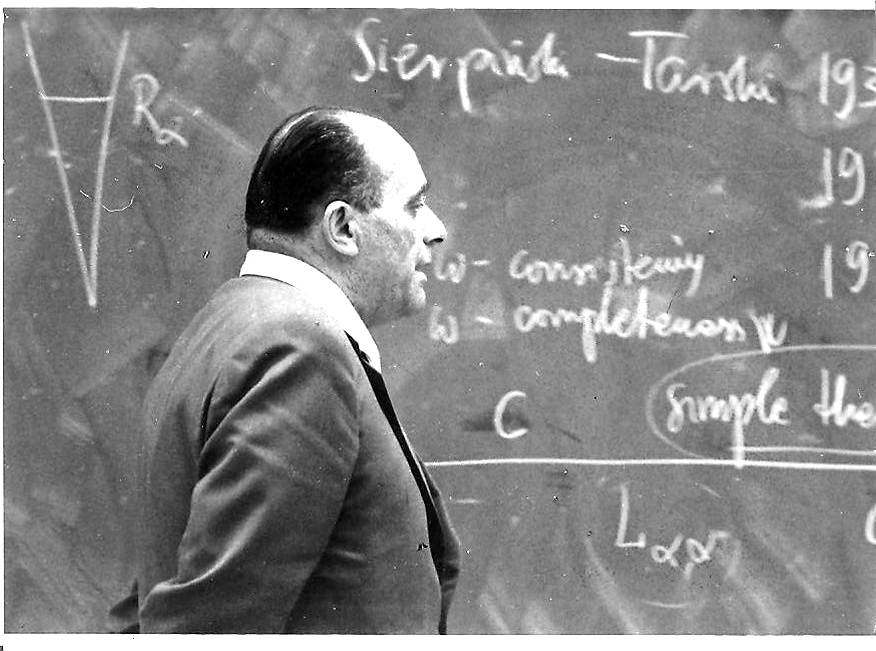
\includegraphics[width=5cm]{AndrzejMostowski73}
\caption{{\tiny przykładowy rysunek - prof. Andrzej Mostowski (1973)}}
\end{figure}
\end{column}


\begin{column}{0.5\textwidth}

\textbf{Nagłówek} Treść

\end{column}


\end{columns}
\end{minipage}


\end{frame}
%----------------------------------------------------------------------------
\begin{frame}{Opis slajdu}
\begin{center}
Polska Cyfrowa Biblioteka Matematyczna \\

\url{http://pldml.icm.edu.pl/}

\begin{figure}[!b]
\centering
\captionsetup{justification=centering}
\captionsetup{labelformat=empty}
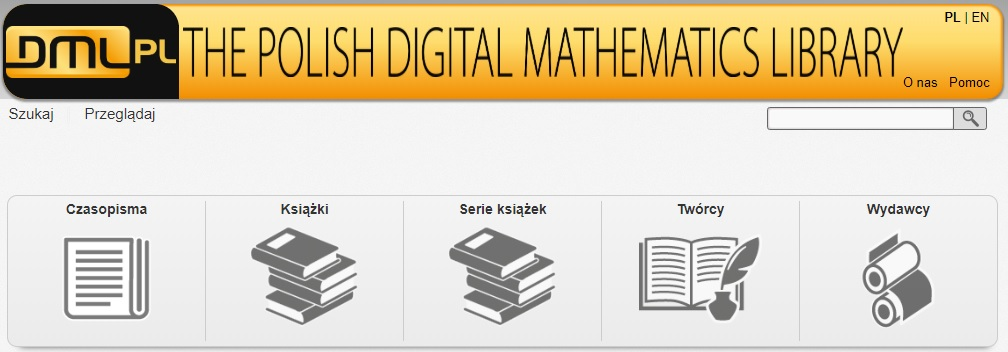
\includegraphics[width=6cm]{DML}
\caption{{\tiny fragment strony Polskiej Cyfrowej Biblioteki Matematycznej}}
\end{figure}

\end{center}

\end{frame}
%----------------------------------------------------------------------------
\begin{frame}{Tytuł slajdu}
\begin{minipage}[0.5\textheight]{\textwidth}
\begin{columns}[T]
\begin{column}{0.5\textwidth}
\begin{figure}
\centering
\captionsetup{justification=centering}
\captionsetup{labelformat=empty}

\includegraphics[width=3cm]{logika_matematyczna}
\caption{{\tiny Strona tytułowa podręcznika autorstwa prof. Mostowskiego}}
\end{figure}
\end{column}

\begin{column}{0.5\textwidth}
\vspace{5mm}
Autor, \\{\it ,,Tytuł''}, \\Wydawnictwo, miasto, rok \\


\end{column}

\end{columns}
\end{minipage}

\end{frame}
%----------------------------------------------------------------------------
\begin{frame}{Elementy logiki}
\begin{center}
{\small
\textbf{,,Motto''} \\ - {\it Źródło} \\
\vspace{2mm}
}

\begin{minipage}[0.2\textheight]{\textwidth}
\begin{columns}[T]
\begin{column}{0.2\textwidth}
\begin{figure}[!b]
\centering
\captionsetup{justification=centering}
\captionsetup{labelformat=empty}
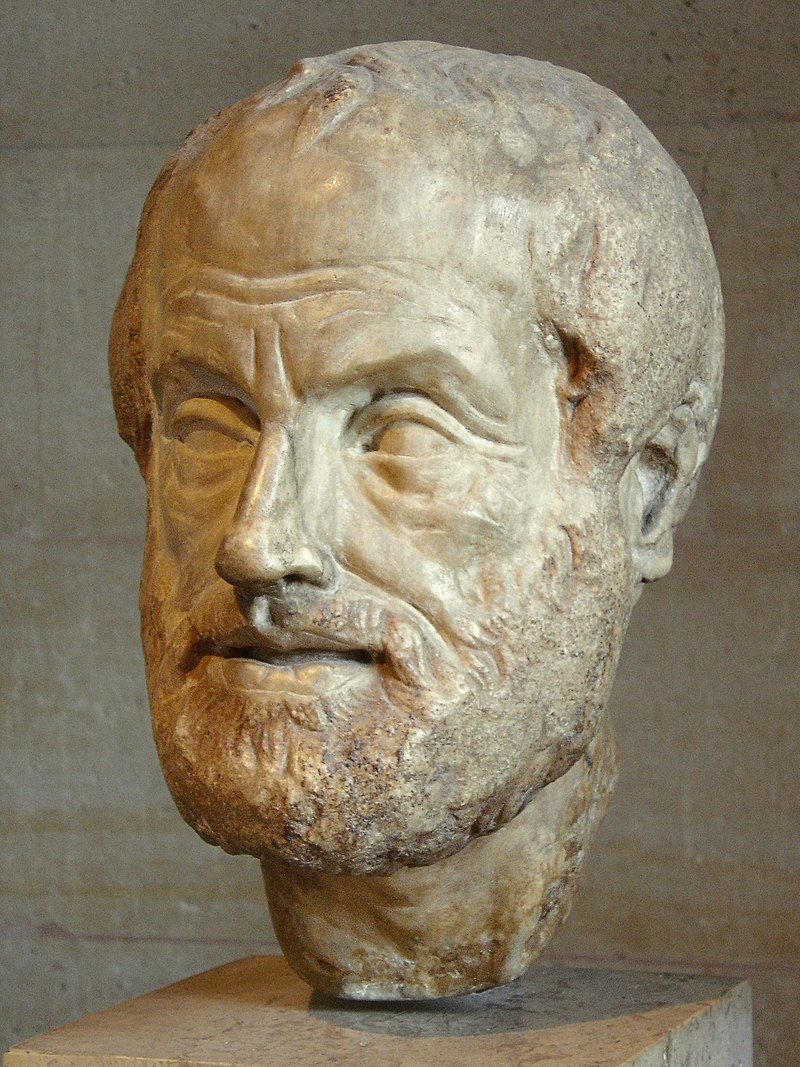
\includegraphics[width=2cm]{800px-Aristoteles_Louvre}
\caption{{\tiny Arystoteles \\384-322 p.n.e.}}
\end{figure}
\end{column}
\begin{column}{0.8\textwidth}
%\begin{itemize}[<+->]
\begin{itemize}
{\small
\item treść
\item treść
\item treść
}
\end{itemize}
\end{column}
\end{columns}
\end{minipage}

\end{center}
\end{frame}

%----------------------------------------------------------------------------

\begin{frame}{Tytuł slajdu}

\begin{small}
Tekst
\begin{itemize}
\item tekst 
\item tekst
\end{itemize}

\vspace{1mm}

Tekst

\begin{itemize}
\item tekst\\ 
\item tekst\\
\end{itemize}

\end{small}
\end{frame}
%----------------------------------------------------------------------------

\begin{frame}{Tytuł slajdu}
\begin{small}
Treść \\

\vspace{3mm}
Treść
\vspace{3mm}

\textbf{,,Cytat''} \\- {\it Źródło}
\end{small}
\end{frame}
%----------------------------------------------------------------------------

\begin{frame}{Tytuł slajdu}
\begin{small}
Jakaś treść. \\
\vspace{3mm}
Jakaś treść.
\end{small}
\end{frame}

%----------------------------------------------------------------------------
%nowa sekcja
%----------------------------------------------------------------------------
\section{Kolejna sekcja}
%----------------------------------------------------------------------------
\begin{frame}{Kolejna sekcja}
treść
\end{frame}
%----------------------------------------------------------------------------
%nowa sekcja
%----------------------------------------------------------------------------
\section{Kolejna sekcja}
%----------------------------------------------------------------------------
\begin{frame}{Kolejna sekcja}
treść
\end{frame}
%----------------------------------------------------------------------------
%nowa sekcja
%----------------------------------------------------------------------------

\section{Kolejna sekcja}
%----------------------------------------------------------------------------
\begin{frame}{Kolejna sekcja}
treść
\end{frame}
%----------------------------------------------------------------------------
%nowa sekcja
%----------------------------------------------------------------------------





\end{document}